\documentclass{jsarticle}

\usepackage[top=30mm, bottom=36mm, left=28mm, right=28mm]{geometry}
\usepackage[yyyymmdd]{datetime}
\usepackage[dvipdfmx]{graphicx}
\usepackage{amsmath,amssymb,amsthm}

\usepackage{../common/mytitle}

\title{データ解析特論 第8回}
\author{201720690 小松 弘人}
\date{\today}
\pagestyle{empty}

\makeatletter
\def\mojiparline#1{
    \newcounter{mpl}
    \setcounter{mpl}{#1}
    \@tempdima=\linewidth
    \advance\@tempdima by-\value{mpl}zw
    \addtocounter{mpl}{-1}
    \divide\@tempdima by \value{mpl}
    \advance\kanjiskip by\@tempdima
    \advance\parindent by\@tempdima
}
\makeatother
\def\linesparpage#1{
    \baselineskip=\textheight
    \divide\baselineskip by #1
}

\begin{document}
\maketitle
\thispagestyle{empty}
\section{課題1}
\subsection{問題}
時間的、あるいは空間的構造を有するデータを用いて回帰を行うことを考える。
このようなデータは独立性を持たず、単純にランダムサンプリングを行うことで
データが有する構造が破壊されてしまう。
この時、クロスバリデーションをどのように行えばよいか考察せよ。

\subsection{回答}
leave-one-outクロスバリデーション (LOOCV) を行うことを考える。
LOOCVは、データセットから1つのデータを取り出してテストデータとし、
それ以外のデータを訓練データとして用いる検証である。
時間的構造を持つデータであれば、テストデータとしてデータを1つ選択し、
それよりも前のデータのみから一定数データを取り出し訓練データとして用いる。
すなわち、過去のデータ (訓練データ) から回帰によって
選択したテストデータを推測できるかどうかを検証する。
これを、全てのデータに対して検証を行うと同時に
検証ごとのデータセットの時系列や訓練データ数といった条件をそろえることによって
時間的構造を破壊することなく検定が行えると考える (図\ref{img:overview})。

また、空間的構造を持つデータにおいても、テストデータとしてデータを1つ選択し、
その周囲の一定範囲のデータを訓練データとすることで
空間的構造を破壊することなく検定が行えると考える。

\begin{figure}[b]
    \centering
    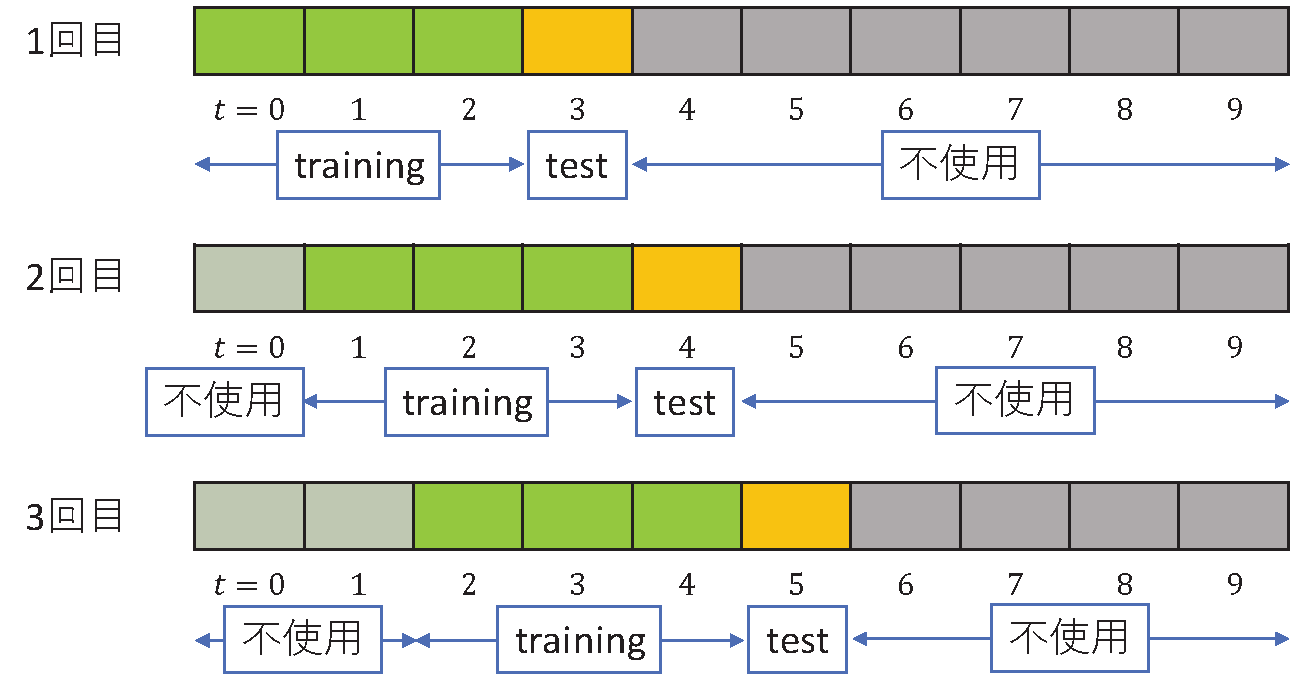
\includegraphics[width=.6\linewidth]{img/loocv.pdf}
    \caption{時間的構造を考慮したクロスバリデーション (説明変数数: 3)}
    \label{img:overview}
\end{figure}

\newpage

\section{課題2}
\subsection{問題}
式\ref{eq:sq_err_ensemble}のアンサンブル学習の二乗誤差のバイアス-分散-共分散分解の式を証明せよ。

\begin{equation}
    err(H) = \bar{b}(H)^2 + \frac{1}{B}\bar{v}(H) + \Bigl(1-\frac{1}{B}\Bigr) \bar{cv}(H)
    \label{eq:sq_err_ensemble}
\end{equation}

\subsection{証明}
\subsubsection{各変数の説明}
アンサンブル学習では、$B$個の仮説$h$を構成する。
$\theta_b$はパラメタである。
$$ {h(x;\theta_b);b=1, \ldots, B} $$
今回は、同じ重みで$B$個の学習機を重ねた平均で予測器$H=\bar{h}$を構成する。
したがって、最終的な仮説$\bar{h}$は式\ref{eq:hypothesis}で構成される。
\begin{equation}
    \bar{h}(x) = \frac{1}{B} \sum_{b=1}^B{h(x;\theta_b)}
    \label{eq:hypothesis}
\end{equation}
平均化バイアス$\bar{b}(H)$、平均化分散$\bar{v}(H)$、平均化共分散$\bar{cv}(H)$は
それぞれ式\ref{eq:mean_bias}、\ref{eq:mean_variance}、\ref{eq:mean_covariance}
のように定義される。
\begin{equation}
    \bar{b}(H)=\frac{1}{B}\sum_{i=1}^B{(E[h_i]-y)}
    \label{eq:mean_bias}
\end{equation}
\begin{equation}
    \bar{v}(H)=\frac{1}{B}\sum_{i=1}^B{E[(h_i-E[h_i])^2]}
    \label{eq:mean_variance}
\end{equation}
\begin{equation}
    \bar{cv}(H)=\frac{1}{B(B-1)}\sum_{i=1}^B\sum_{j=1,j\neq i}^B{E[(h_i-E[h_i])]E[(h_j-E[h_j])]}
    \label{eq:mean_covariance}
\end{equation}

また、一般的な機械学習の平均二乗誤差は式\ref{eq:sq_err_basis}のように表される。
\begin{equation}
    err(h)=E[(h-y)^2]=(E[h]-y)^2+E[(h-E[h])^2]=b(h)^2+v(h)
    \label{eq:sq_err_basis}
\end{equation}
ただし、$b(h)$はバイアス、$v(h)$は分散であり、式\ref{eq:bias}, \ref{eq:variance}のように定義される。
\begin{eqnarray}
    \label{eq:bias}
    b(h)&=&E_{(x)}[h]-y\\
    \label{eq:variance}
    v(h)&=&E[(h-E_X[h])^2]
\end{eqnarray}

\subsubsection{証明}
今回は、式\ref{eq:sq_err_basis}を用いてアンサンブル学習の二乗誤差を求める。
まず、$err(\cdot)$に$H=\bar{h}$を代入する。
\begin{eqnarray}
    err(H) &=& err(\bar{h}) \nonumber \\
    &=& E[(\bar{h}-y)^2] \nonumber \\
    \label{eq:err_expansion}
    &=& (E[\bar{h}]-y)^2+E[(\bar{h}-E[\bar{h}])^2]
\end{eqnarray}

式\ref{eq:err_expansion}の第1項は、式\ref{eq:hypothesis}、\ref{eq:mean_h}より以下のように変形できる。
\begin{equation}
    (E[\bar{h}]-y)^2 = \Biggl\{\frac{1}{B}\sum_{i=1}^B{E[h_i]-\frac{1}{B}\sum_{i=1}^B{y}}\Biggr\}^2 = \Biggl\{\frac{1}{B}\sum_{i=1}^B{(E[h_i]-y)} \Biggr\}^2 = \bar{b}(H)^2
    \label{eq:ensemble_bias}
\end{equation}
\begin{equation}
    E[\bar{h}]=E\Biggl[\frac{1}{B}\sum_{i=1}^B{h_i}\Biggr]=\frac{1}{B}\sum_{i=1}^B{E[h_i]}
    \label{eq:mean_h}
\end{equation}

また、式\ref{eq:err_expansion}の第2項は、式\ref{eq:mean_variance}、\ref{eq:mean_h}より以下のように変形できる。
\begin{eqnarray}
    E[(\bar{h}-E[\bar{h}])^2] &=& E\Biggl[\Biggl\{\frac{1}{B}\sum_{i=1}^B{(h_i-E[h_i])}\Biggr\}^2\Biggr] \nonumber \\
    &=& E\Biggl[\frac{1}{B}\sum_{i=1}^B{(h_i-E[h_i])}\cdot\frac{1}{B}\sum_{j=1}^B{(h_j-E[h_j])}\Biggr] \nonumber \\
    &=& \frac{1}{B^2}\sum_{i=1}^B\sum_{j=1}^B{E[(h_i-E[h_i])(h_j-E[h_j])]} \nonumber \\
    &=& \frac{1}{B^2}\Biggl\{\sum_{i=1}^B\sum_{j=i}^i{E[(h_i-E[h_i])(h_j-E[h_j])]}\Biggr\} \nonumber \\
    &+& \frac{1}{B^2}\sum_{i=1}^B\sum_{j=1,j\neq i}^B{E[(h_i-E[h_i])(h_j-E[h_j])]} \nonumber \\
    &=& \frac{1}{B}\Biggl\{\frac{1}{B}\sum_{i=1}^B{E[(h_i-E[h_i])^2]}\Biggr\}\!+\!\frac{1}{B^2}\sum_{i=1}^B\sum_{j=1,j\neq i}^B{E[(h_i-E[h_i])(h_j-E[h_j])]} \nonumber \\
    \label{eq:2nd_expansion}
    &=& \frac{1}{B}\bar{v}(H)+\frac{1}{B^2}\sum_{i=1}^B\sum_{j=1,j\neq i}^B{E[(h_i-E[h_i])(h_j-E[h_j])]}
\end{eqnarray}

$h_i$はそれぞれ独立した仮説であり共分散は0であるため、式\ref{eq:mean_covariance}より式\ref{eq:2nd_expansion}の第2項は以下のように変形できる。
\begin{eqnarray}
    \frac{1}{B^2}\sum_{i=1}^B\sum_{j=1,j\neq i}^B{E[(h_i-E[h_i])(h_j-E[h_j])]} &=& \frac{1}{B^2}\sum_{i=1}^B\sum_{j=1,j\neq i}^B{E[(h_i-E[h_i])]E[(h_j-E[h_j])]} \nonumber \\
    &=& \frac{B-1}{B}\frac{1}{B(B-1)}\sum_{i=1}^B\sum_{j=1,j\neq i}^B{E[(h_i-E[h_i])]E[(h_j-E[h_j])]} \nonumber \\
    &=& \Bigl(1-\frac{1}{B}\Bigr)\frac{1}{B(B-1)}\sum_{i=1}^B\sum_{j=1,j\neq i}^B{E[(h_i-E[h_i])]E[(h_j-E[h_j])]} \nonumber \\
    \label{eq:ensemble_covariance}
    &=& \Bigl(1-\frac{1}{B}\Bigr)\bar{cv}(H)
\end{eqnarray}

式\ref{eq:2nd_expansion}、\ref{eq:ensemble_covariance}より、以下の式が得られる。
\begin{eqnarray}
    \label{eq:ensemble_2nd}
    E[(\bar{h}-E[\bar{h}])^2] &=& \frac{1}{B}\bar{v}(H)+ \Bigl(1-\frac{1}{B}\Bigr)\bar{cv}(H)
\end{eqnarray}

よって、式\ref{eq:ensemble_bias}、\ref{eq:ensemble_2nd}より、式\ref{eq:sq_err_ensemble}が得られる。
\begin{eqnarray}
    err(H) &=& (E[\bar{h}]-y)^2+E[(\bar{h}-E[\bar{h}])^2] \nonumber \\
    &=&  \bar{b}(H)^2 + \frac{1}{B}\bar{v}(H)+ \Bigl(1-\frac{1}{B}\Bigr)\bar{cv}(H) \nonumber
\end{eqnarray}

\qed

\end{document}
